\subsection{Integration}
The current phase of the project considers itself as the most programming-heavy one.
In the best case, it will focus on integrating all the parts in one C\# language-based environment.
In the worst case~\footnote{as, it became already}; it may become combinations of Python, C\# and bash.
However, the first workable results are present here.\\[1pc]
The goal is to adapt whatever discovery to the hardware in hand and integrate it with the Game Engine.
So far, only camera usage and object detection can provide reliable results.
By the end of the project, all other parts will have something more efficient to present.
\subsubsection{$360\circ$ camera}
There are several ways of using this IP address in Unity Advantage.
The investigation part comes with three modes, Skybox, around a box and a sphere.\\
The first method may sound tempting but far from the overall goal.
The whole sky becomes one large video file.
It is hardly a solution to the current problem. \\
Using Unity Extension called \textit{EasyMovieTexture}, the integration video stream with an object was a success.
Output different angles on a square frame allowed to produce five areas with video files shown during the play-through. \\
A sphere one using a similar extension had better results.
It can both accept a video stream or prerecorded file; the images and demos are located in further sections.
\subsubsection{Object Detection \& Machine Learning Nets}
OpenCV integration and colour detection were only the first step.
A TensorFlow plugin allows to integration of more complicated calculations into the project, for example, performing real-time detection, 
An easy and straightforward Mobile Net model already presented out of the box.
It helps to classify various objects from its' databases.
After performing certain pretraining with more tank-based data, it should be able to detect enemies, potential targets or other objects of interest.
The table in Appendix~\ref{fig:keras} represents official model benchmarks from Keras website~\cite{noauthor_applications_2018}.
Speed is a primary criterion for this project, which is why mobile net or other similar branches are going to be a priority in implementation.
\subsubsection{Unity Game Engine}
After completing and testing the first part of the planned work over the initial stages of the report, it was decided to move the project into a new version of Unity.
The entire project was rebuilding from the start using version 2018.3.1f1 and will remain the same until the end.
As a result, some of the assets required reimporting and some additional configured:
\begin{enumerate}
    \item \textbf{Ground Texture Pack:} To give surrounding area proper look.
    \item \textbf{T34 Tank Model:} A first testing Tank model.
    \item \textbf{QUT Tank Model:} Prefab, developed by Rodney Zsolczay.
    \item \textbf{Tileable Pack 01 (MAFUBASH):} An extra prefab
    \item \textbf{EasyMovieTexture V 3.69:} Upon moving to the new version and with new hardware, the older version appeared to be nonfunctional anymore.\footnote{Problems occurred around FFmpeg and AVformat library. Unfortunately, that was one of the issue updating to the latest version of Unity}
    \item \textbf{ML-Agents:} Plugin for using Machine Learning in Unity with Tensorflow-Csharp.
    \item \textbf{NetMQExample:} Used for socket communication with ZMQ Library
    \item \textbf{SteamVR:} Prefab used by HTC Vive to create a Virtual Reality Experience
\end{enumerate}
The next part will cover some of them in detail.
They are meant to bring clarity to the application and usage.
\begin{enumerate}
    \item \textbf{VR gear and SteamVR} \\
    HTC and Valve designed those tools for smooth integration with Unity.
    Their usage, limitations and type of suitable devices will be acknowledged later after presenting the first playable product.
    So far, SteamVR prefab and belonging documentation suited the overall project very well. 
    It caused no problem to apply it with HTC Vive, unlike PIXPRO in the section above. 
    The reason behind adding extra library support is manipulation with controllers. 
    The event system triggering has proven to be effective, though very different from every released version.
    It caused another development issue, which requires a separate and significant amount of time to study API.
    \item \textbf{EasyMovieTexture usage} \\
    It was an unfortunate coincidence that Version of Windows managed to update itself to latest without users notice, which lead to some incompatibility errors.\footnote{Take Away from this accident is -  NEVER work with Windows. 
    The next Unity project will work in a Linux environment. Even if it meant to use Wine HQ.} 
    The old version of the movie Texture had a significant issue upon running. 
    It may be relevant either to new hardware or new system configuration. 
    As a result, EasyMovieTeture required an update to the latest in order to support the UDP protocol stream received from FFmpeg.
    After that, usage of that prefab is only based on the given input and expected output.
    The streaming script is very adaptable and can be easily integrated into other components of the project.
    \item \textbf{FFmpeg AutoGen} \\
    The tool is designed to be integrated into Unity as a prefab, to use some of the Libraries with the power of Unity.
    It allows some simple video operation.
    However, this turned out to be not enough to discover a way to resolve the issue with the Video stream.
    In order to make changes, the library required manual recompilation.
    The effort and library management turned out to be too ineffective compared to how much it was spent with Tensorflow and from experience.
    Therefore FFmpeg was used outside of Unity to capture a video stream and to modify before entering Unity.
    The latest build from the official website provided all the necessary means.
    Details are followed in the Design section.
    \item \textbf{ML Agents} \\
    Machine Learning Agents Prefab was used to test first encounters with learned model usage.
    Some test scripts provided an excellent example of how to perform more complicated training, like balancing spheres, Figure~\ref{fig:ML-balancing} on a surface with varying gravity levels.
    The one which this project focuses on is Image recognition~\cite{unity-technologies_unity_2019}.
    It was designed to run on Android camera devices.
    However, using the TF-NetSharp library, it was a matter of time and skill to reapply learned configurations to the new environment. 
    As a result, with a trained Mobile Net model, Unity was able to recognise some of the surrounding objects.
    The next part will cover some of them in detail. 
    They are meant to bring clarity to the application and usage.
    \begin{figure}[H]
		\centering
		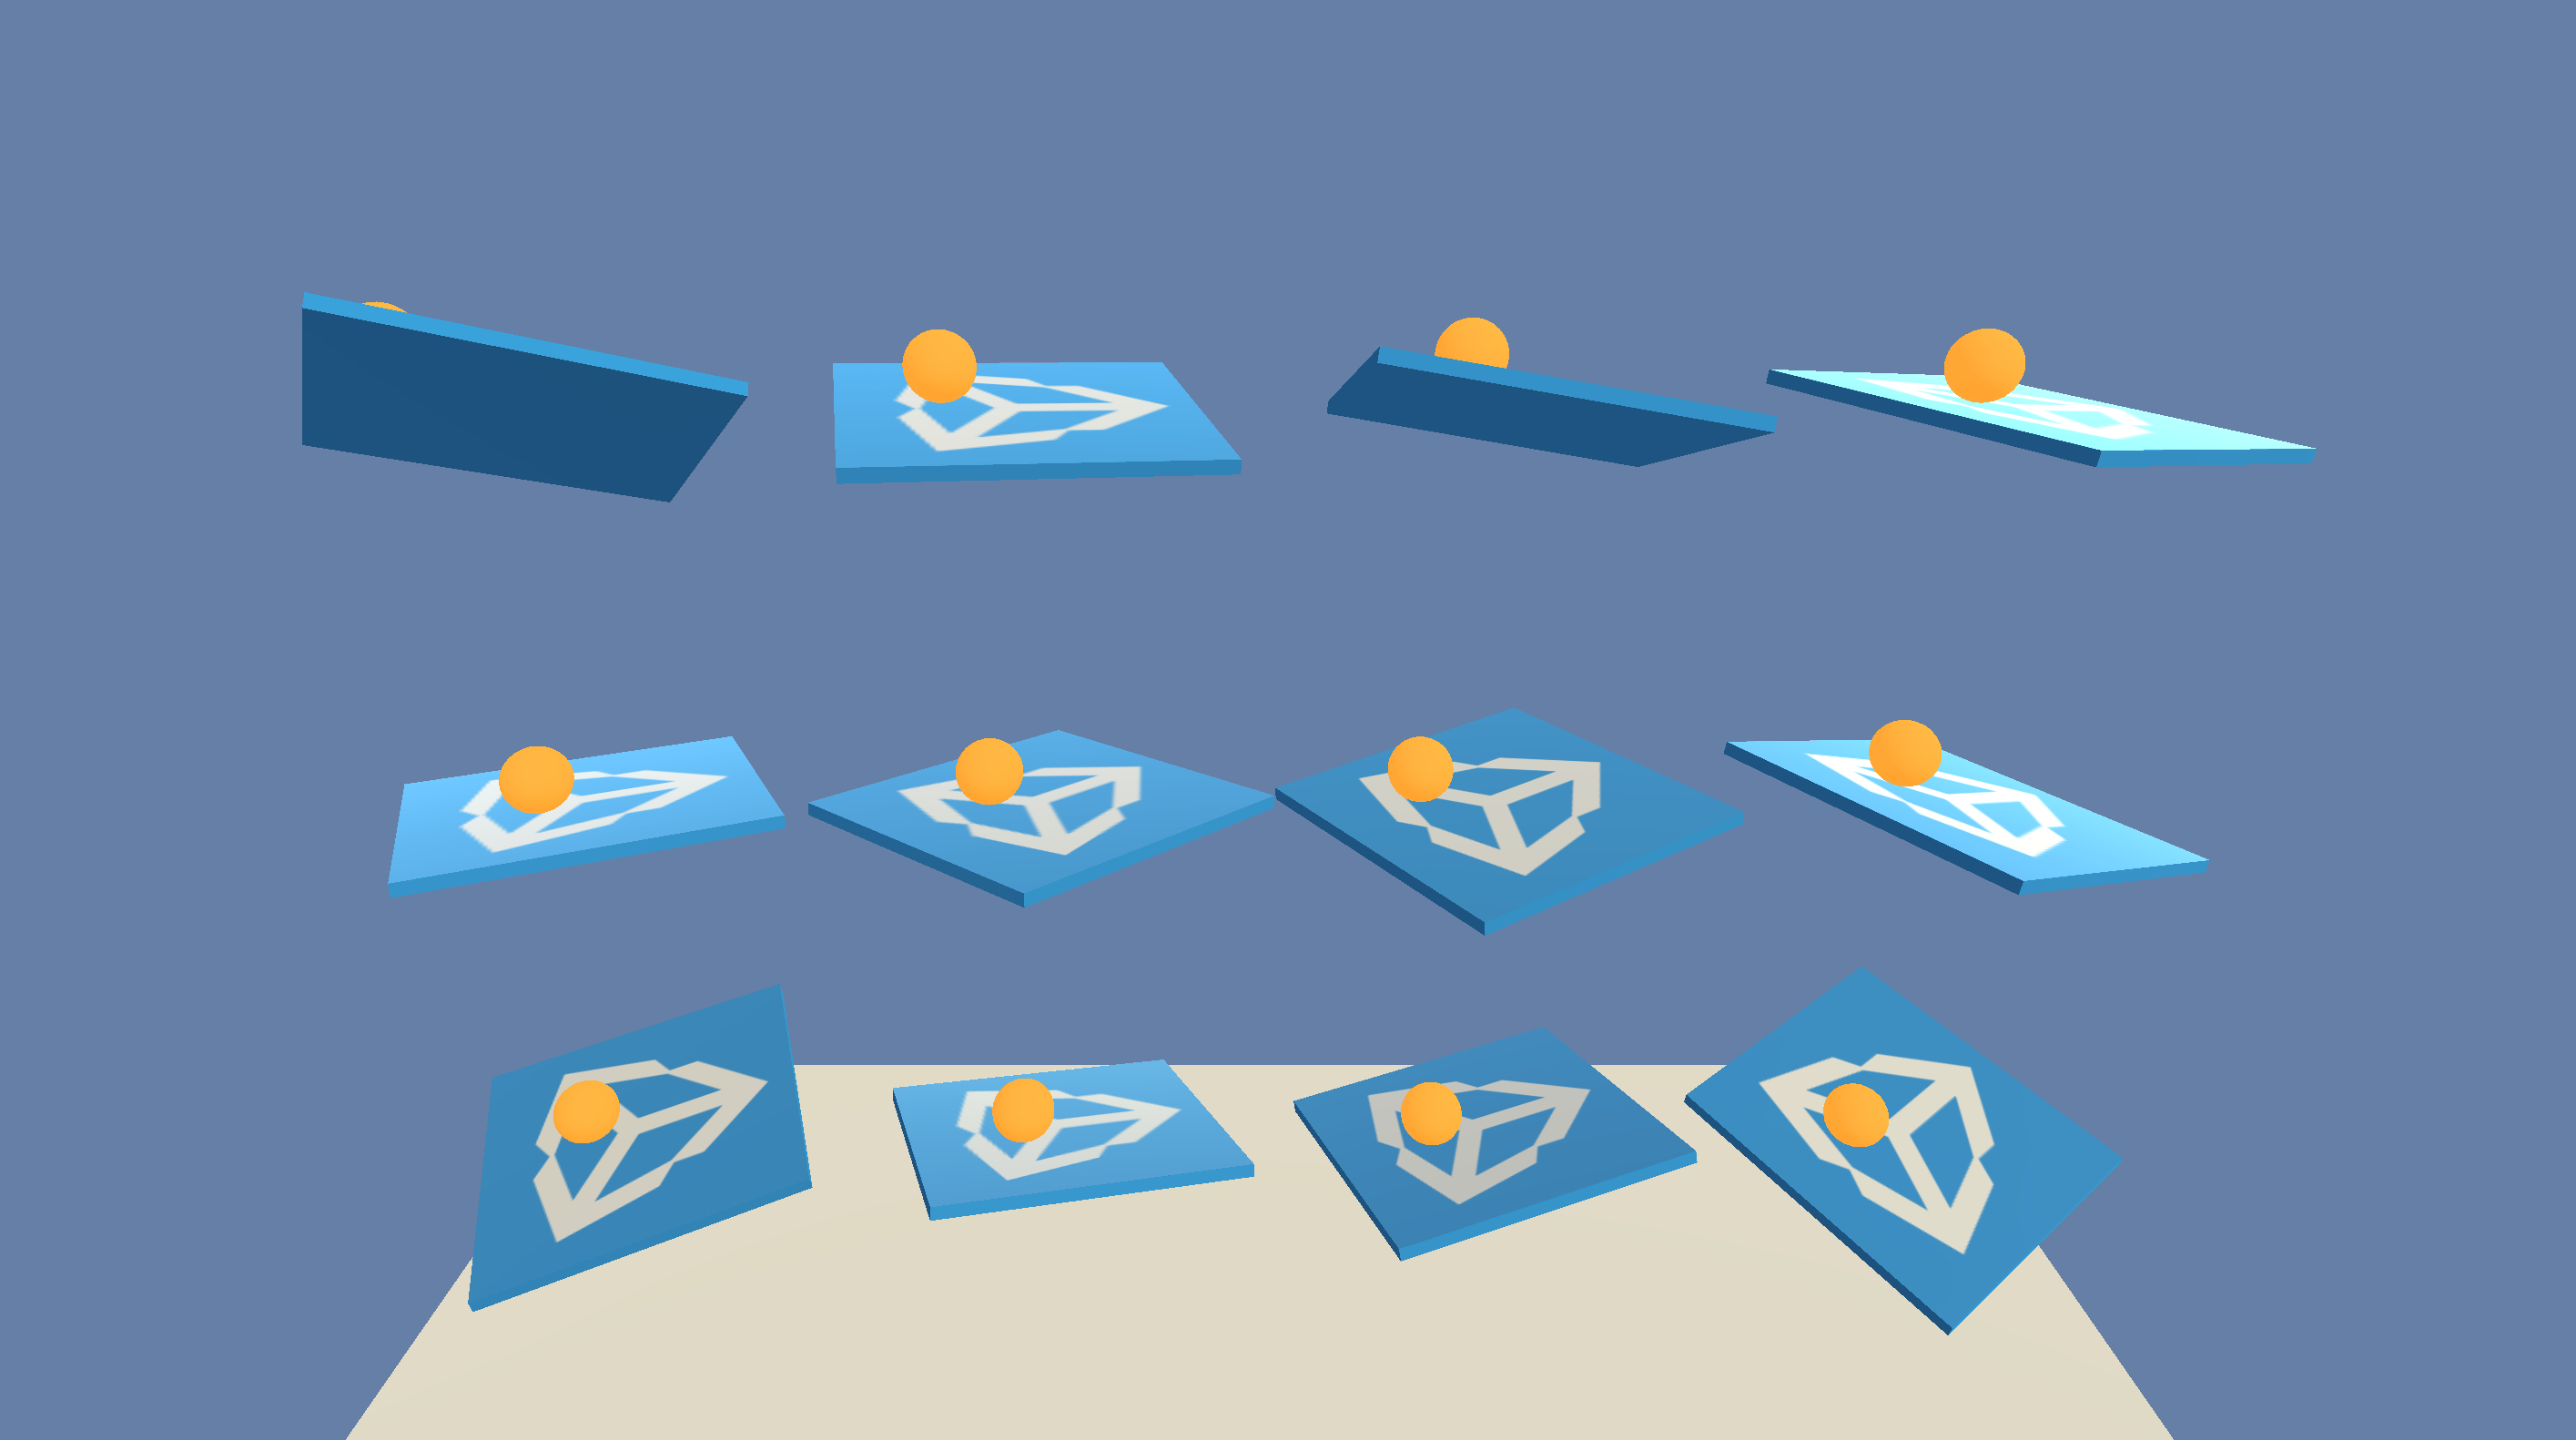
\includegraphics[width=0.5\linewidth]{project/images/balance.png}
		\caption{ML balancing example}
		\label{fig:ML-balancing}
	\end{figure}
\end{enumerate}